%%%%%%%%%%%%%%%%%%%%%%%%%%%%%%%%%%%%%%%%%%%%%%%%%%%%%%%%%%%%%%%%
%%                                                            %%
%% aGreekPrimer, Italian translation 2016.12 - 2017           %%
%%                                                            %%
%% From:  Clarence W. Gleason, A Greek Primer                 %%
%%        (1903, New York, American Book Company)             %%
%%                                                            %%
%%        https://archive.org/details/greekprimer00glea       %%
%%                                                            %%
%% Translated by g.p.ciceri <gp.ciceri@gmail.com>             %%
%% ---------------------------------------------------------- %%
%% This translation is Licensed under                         %%
%% Creative Commons Attribution-ShareAlike 4.0 International  %%
%% https://creativecommons.org/licenses/by-sa/4.0/            %%
%%                                                            %%
%%%%%%%%%%%%%%%%%%%%%%%%%%%%%%%%%%%%%%%%%%%%%%%%%%%%%%%%%%%%%%%%

% ᾶῖῶῆῦ  
% ἀἰὐἐὀὠἠ 
% ὰὲὶὸὺὼὴ 
% ἁἱὑὁὡἡῥ
% άέίόύήώΆΉ
% ἂἒὒἲὂὢἢὒἚἊ
% ἃἳὓὃἣὣἓἋἛ
% ἄἔἴὄὔὤἤἌἬ
% ἅἕἵὅὕὥἥἍἭ
% ἆὦἶἦὖἯἏὯἇὧἷἧὗἯἏὯ 

% ᾳῃῳ
% ᾱῑῡ
% ᾀᾐᾠ
% ᾰῐῠ
% ᾂᾒᾢ
% ϊ ϋ
% ᾄᾔᾤ
% ΰ ΐ
% ᾆᾖᾦ
% ᾲῂῲ
% ᾴῄῴ
% ᾷῇῷ


\documentclass[nols]{tufte-handout}

%\geometry{showframe} % display margins for debugging page layout

\usepackage{fontspec}
\usepackage{ifxetex}
\setmainfont[Path=./fonts/palatino-linotype/, ItalicFont=palai.ttf, BoldFont=palab.ttf]{pala.ttf}


% \defaultfontfeatures{Mapping=tex-text}
% \setromanfont[Path=./fonts/TeX-Gyre-Schola/,Mapping=tex-text]{TeX Gyre Schola}
% \setsansfont[Path=./fonts/TeX-Gyre-Heros/,Scale=MatchLowercase,Mapping=tex-text]{TeX Gyre Heros}
% \setmonofont[Path=./fonts/TeX-Gyre-Cursor/,Scale=MatchLowercase]{TeX Gyre Cursor}

\usepackage{lipsum}
\usepackage{url}
\usepackage{longtable}
\usepackage{stackengine}

\usepackage{graphicx} % allow embedded images
  \setkeys{Gin}{width=\linewidth,totalheight=\textheight,keepaspectratio}
  \graphicspath{{graphics/}} % set of paths to search for images
\usepackage{amsmath}  % extended mathematics
\usepackage{booktabs} % book-quality tables
\usepackage{units}    % non-stacked fractions and better unit spacing
\usepackage{multicol} % multiple column layout facilities
\usepackage{lipsum}   % filler text
\usepackage{fancyvrb} % extended verbatim environments
  \fvset{fontsize=\normalsize}% default font size for fancy-verbatim environments

% Standardize command font styles and environments
\newcommand{\doccmd}[1]{\texttt{\textbackslash#1}}% command name -- adds backslash automatically
\newcommand{\docopt}[1]{\ensuremath{\langle}\textrm{\textit{#1}}\ensuremath{\rangle}}% optional command argument
\newcommand{\docarg}[1]{\textrm{\textit{#1}}}% (required) command argument
\newcommand{\docenv}[1]{\textsf{#1}}% environment name
\newcommand{\docpkg}[1]{\texttt{#1}}% package name
\newcommand{\doccls}[1]{\texttt{#1}}% document class name
\newcommand{\docclsopt}[1]{\texttt{#1}}% document class option name
\newenvironment{docspec}{\begin{quote}\noindent}{\end{quote}}% command specification environment

% concetti morfosintattici
\usepackage{xspace} 
\newcommand{\noun}{\textsc{sostantivo}\xspace}
\newcommand{\nouns}{\textsc{sostantivi}\xspace}
\newcommand{\adject}{\textsc{aggettivo}\xspace}
\newcommand{\adjects}{\textsc{aggettivi}\xspace}
\newcommand{\gnumber}{\textsc{numero}\xspace}
\newcommand{\gnumbers}{\textsc{numeri}\xspace}
\newcommand{\gender}{\textsc{genere}\xspace}
\newcommand{\genders}{\textsc{generi}\xspace}
\newcommand{\gcase}{\textsc{caso}\xspace}
\newcommand{\gcases}{\textsc{casi}\xspace}
\newcommand{\tense}{\textsc{tempo}\xspace}
\newcommand{\mood}{\textsc{modo}\xspace}
\newcommand{\gverb}{\textsc{verbo}\xspace}
\newcommand{\gverbs}{\textsc{verbi}\xspace}
\newcommand{\adjective}{\textsc{aggettivo}\xspace}
\newcommand{\nom}{\textsc{nom}\xspace}
\newcommand{\gen}{\textsc{gen}\xspace}
\newcommand{\dat}{\textsc{dat}\xspace}
\newcommand{\acc}{\textsc{acc}\xspace}
\newcommand{\voc}{\textsc{voc}\xspace}
\newcommand{\gexit}{\textsc{uscita}\xspace}
\newcommand{\gexits}{\textsc{uscite}\xspace}
\newcommand{\declinazione}{\textsc{declinazione}\xspace}
\newcommand{\masc}{\textsc{maschile}\xspace}
\newcommand{\femm}{\textsc{femminile}\xspace}
\newcommand{\neut}{\textsc{neutro}\xspace}

\newcommand{\indic}{\textsc{indicativo}\xspace}
\newcommand{\imper}{\textsc{imperativo}\xspace}
\newcommand{\gcong}{\textsc{congiuntivo}\xspace}
\newcommand{\ott}{\textsc{ottativo}\xspace}
\newcommand{\partic}{\textsc{participio}\xspace}
\newcommand{\infin}{\textsc{infinito}\xspace}

\newcommand{\pres}{\textsc{presente}\xspace}
\newcommand{\imperf}{\textsc{imperfetto}\xspace}
\newcommand{\aor}{\textsc{aoristo}\xspace}
\newcommand{\fut}{\textsc{futuro}\xspace}

\newcommand{\sing}{\textsc{singolare}\xspace}
\newcommand{\plur}{\textsc{plurale}\xspace}
\newcommand{\dual}{\textsc{duale}\xspace}


% italianitudini
\renewcommand{\figurename}{Figura}
\renewcommand{\tablename}{Tabella}
\renewcommand{\contentsname}{Indice}

% fix per un qualche problema
\ifxetex
  \newcommand{\textls}[2][5]{%
    \begingroup\addfontfeatures{LetterSpace=#1}#2\endgroup
  }
  \renewcommand{\allcapsspacing}[1]{\textls[15]{#1}}
  \renewcommand{\smallcapsspacing}[1]{\textls[10]{#1}}
  \renewcommand{\allcaps}[1]{\textls[15]{\MakeTextUppercase{#1}}}
  \renewcommand{\smallcaps}[1]{\smallcapsspacing{\scshape\MakeTextLowercase{#1}}}
  \renewcommand{\textsc}[1]{\smallcapsspacing{\textsmallcaps{#1}}}
\fi

\title{A Greek Primer. Introduzione al Greco Antico \newline Lezione VI - L'aoristo indicativo attivo.}

\author[gpciceri]{a cura di Milagathòs: Milo's help to enjoy humanities\marginnote{\url{http://www.milagathos.com}}
}

\date{1 Gennajo 2017} % without \date command, current date is supplied


\begin{document}

\maketitle% this prints the handout title, author, and date

\begin{marginfigure}[-2.5cm]
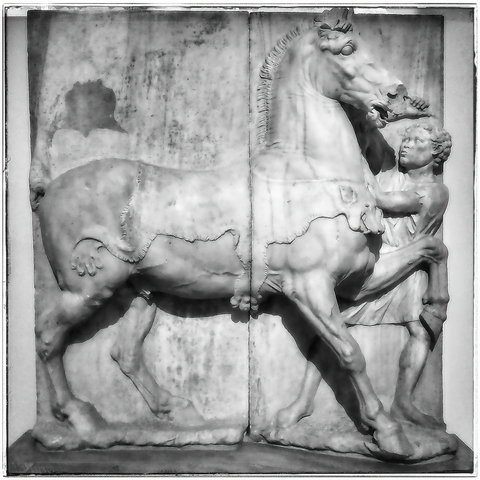
\includegraphics{smallthumb-lesson_I.jpeg}
\setfloatalignment{b}
\end{marginfigure}


\begin{abstract}
\noindent
Queste lezioni si articolano in \textsc{elementi grammaticali}, 
espressi sommariamente, seguiti da \textsc{vocabolari} per il lessico di base 
e da \textsc{frasi da tradurre} dal greco e in greco. 
\
L'approccio è quello del testo-laboratorio di morfosintassi: 
si presenta punto per punto - riprendendone la numerazione - 
l'esposizione di Gleason\cite{gleason1903}.\\
\bigskip
\noindent
Lezione VI: l'aoristo indicativo attivo, aoristo primo e secondo, regola di sintassi: concordanza del soggetto neutro plurale con in verbo al singolare, esercizi.
\end{abstract}

%\printclassoptions

\newthought{81.} L'aoristo indica un'azione compiuta in un tempo passato, come in \textbf{ἔλυσα}, \textit{io sciolsi}. Nella maggior parte dei verbi l'aoristo attivo si forma aggiungendo \textbf{σα} al tema del verbo, come in \textbf{ἔλυ-σα}.

\newthought{82.} Alcuni verbi hanno un aoristo più semplice e primitivo, formato dal tema verbale e coniugato come l'imperfetto, come in \textbf{ἔβαλον}, \textit{io gettai} da \textbf{βάλλω} (tema \textbf{βαλ-}), imperfetto \textbf{ἔβαλλον}; da \textbf{λείπω} (tema \textbf{λιπ-}), imperfetto \textbf{ἔλειπον}, aoristo \textbf{ἔλιπον}.

\newthought{83. Aoristo primo e secondo} Per convenienza, gli aoristi in \textbf{-σα} sono detti \textbf{aoristi primi}; quelli in \textbf{-ον, aoristi secondi}. Pochi verbi presentano tutte e due le forme.

\newthought{84. L'aoristo Indicativo Attivo}

\begin{fullwidth}
\begin{table}[!htbp]
  \centering
  \begin{tabular}{l l l l l l}
    %\toprule
	\multicolumn{6}{c}{\textsc{coniugazione dell'aoristo indicativo attivo}} \\
	\multicolumn{3}{c}{\textbf{λύω}} & \textbf{πέμπω} & \textbf{λείπω} & \textbf{βάλλω} \\
    %\midrule
	& \multicolumn{4}{c}{\textsc{singolare}} \\
    \textsc{1.} & \textbf{ἔλυσα}   & \textit{io sciolsi}    & \textbf{ἔπέμψα}  & \textbf{ἔλιπον}  & \textbf{ἔβαλον} \\
    \textsc{2.} & \textbf{ἔλυσας}   & \textit{tu sciogliesti}    & \textbf{ἔπέμψας} & \textbf{ἔλιπες}  & \textbf{ἔβαλες} \\
    \textsc{3.} & \textbf{ἔλυσε}    & \textit{egli sciolse} & \textbf{ἔπέμψε}  & \textbf{ἔλιπε}   & \textbf{ἔβαλε} \\
	 & \multicolumn{4}{c}{\textsc{plurale}}  \\
	\textsc{1.} & \textbf{ἔλυσαμεν} & \textit{noi sciogliemmo} & \textbf{ἔπέμψαμεν} & \textbf{ἐλίπομεν}   & \textbf{ἔβαλομεν} \\
    \textsc{2.} & \textbf{ἔλυσατε}  & \textit{voi scioglieste} & \textbf{ἔπέμψατε}  & \textbf{ἐλίπετε}  & \textbf{ἔβαλετε} \\
    \textsc{3.} & \textbf{ἔλυσαν}   & \textit{essi sciolsero} & \textbf{ἔπέμψαν} & \textbf{ἔλιπον}  & \textbf{ἔβαλον} \\
    %\bottomrule
  \end{tabular}
  \caption{λύω, πέμπω, λείπω, βάλλω: aoristo indicativo attivo}
  \label{tab:normaltab}
  %\zsavepos{pos:normaltab}
\end{table}
\end{fullwidth}

\newthought{Esercizi}
\begin{itemize}
\item[\textsc{1.}] Coniuga l'aoristo primo di \textbf{παίω, γράφω, ἁρπάζω}.  
\item[\textsc{2.}] Coniuga l'aoristo secondo di \textbf{φεύγω} (tema \textbf{φυγ-}), \textbf{εὑρίσκω} (tema \textbf{εὑρ-}).
\item[\textsc{3. Aoristo di ἄγω e di ἔχω}] L'aoristo di \textbf{ἄγω} è irregolare, fa \textbf{ἤγαγον}. L'aoristo primo \textbf{ἦξα} è raro. \textbf{ἔχω} ha l'aoristo secondo \textbf{ἔσχον.} Coniuga l'aoristo per questi due verbi.
\end{itemize}

\newthought{85. Regola di sintassi} Un soggetto neutro plurale generalmente vuole il verbo coniugato al singolare, come in \textbf{ἦν δὲ πὲντε παιδία,} \textit{vi erano cinque bambini.}

\hyphenation{τέκ-να}
\hyphenation{ἔ-λυ-σαν}
\hyphenation{ἔ-με-νον}

\newthought{86. Traduci:}
\textsc{1.}~ηὗρον λίθους καλοὺς ἐν τῷ πεδίῳ. \quad
\textsc{2.}~τὰ δὲ τέκνα τοῦ ἀγγέλου ἔβαλε\sidenote{cfr. 85.} τοὺς λίθους εἰς τὸν ποταμόν. \quad
\textsc{3.}~ἔσχε δὲ πέντε πλοῖα ἐν τῷ χωρίῳ. \quad
\textsc{4.}~τίς ἔφυγεν\sidenote{\textbf{ν} mobile} ἐκ τοῦ ἱεροῦ; \quad
\textsc{5.}~ἔλυσαν τοὺς ἵππους καὶ ἔπαισαν τοὺς κακοὺς δούλους. \quad
\textsc{6.}~ἤγαγον γὰρ τοὺς ἵππους εἰς τὸ ἱερόν. \quad
\textsc{7.}~τὰ παιδία τοῦ ἀγαθοῦ ἀνθρώπου οὐκ ἦν κακά. \quad
\textsc{8.}~ἐκέλευσε δὲ τὰ παιδία ἄγειν\sidenote{presente infinito attivo.} τὰ ἱμάτια. \quad
\textsc{9.}~ἔμενον δὲ οἱ ἄγγελοι ἐπὶ τοῖς πλοίοις καὶ ἔθυον τοῖς θεοῖς.


\begin{figure}[!b]
  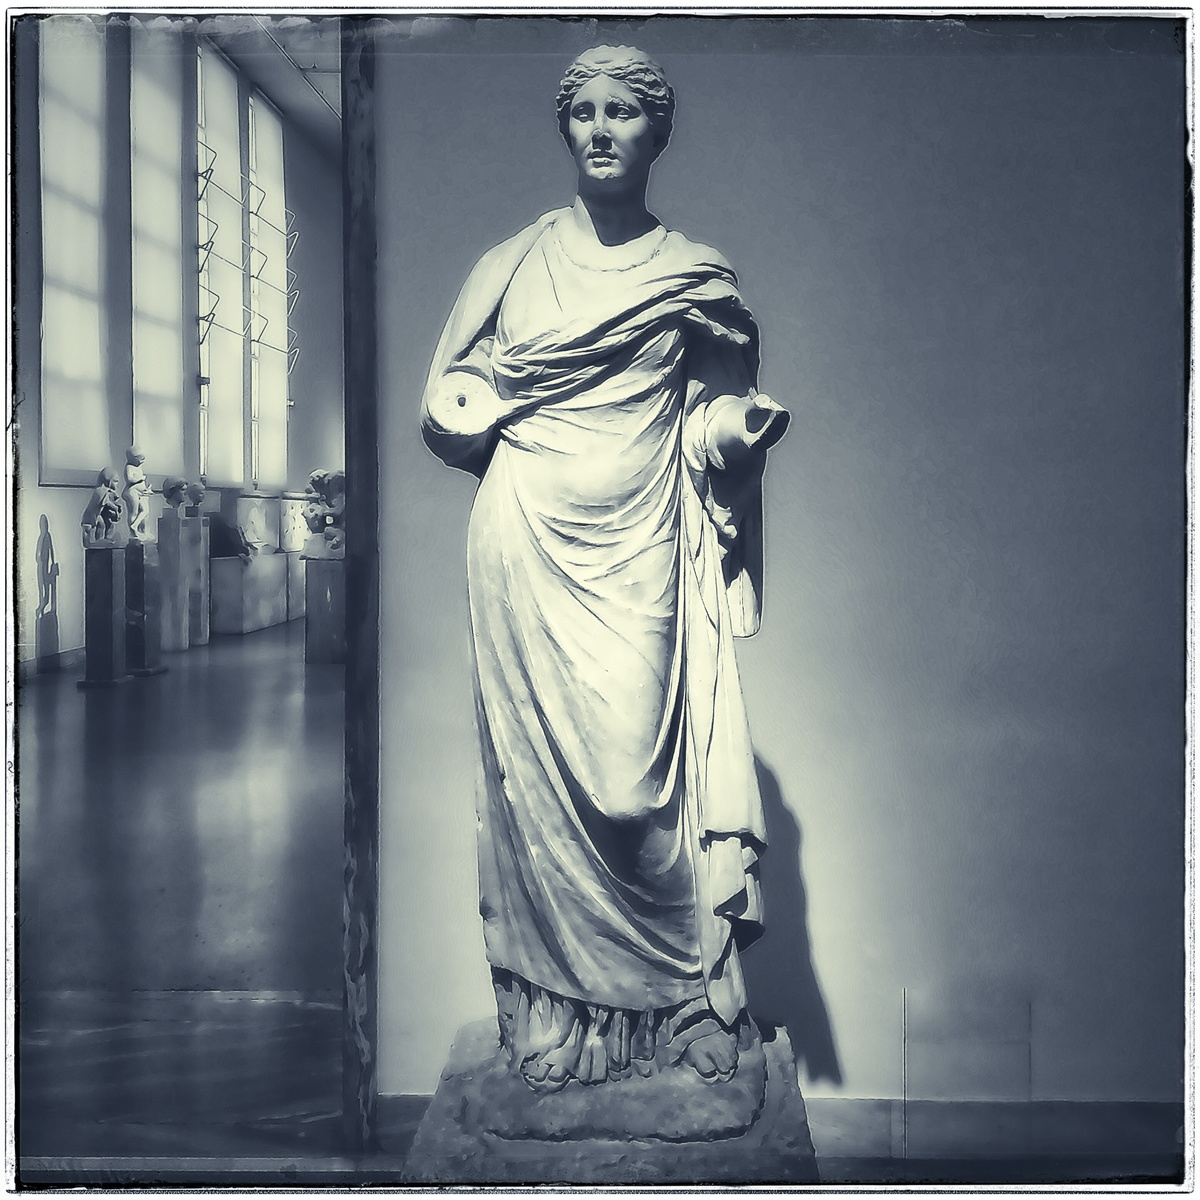
\includegraphics{thumb-lesson_VI.jpeg}
  \caption{Museo Nazionale di Archeologia di Atene}
  \label{fig:textfig}
  %\zsavepos{pos:textfig}
  \setfloatalignment{b}
\end{figure}

\nobibliography{greekBiblio}
\bibliographystyle{alpha}


\end{document}
